\section{Testing and Results}

\subsection{Testing Strategy}
This Chapter details testing methodologies used to verify functional and non-functional aspects of the Master Node, IoT Node, and the Shipment Tracker Contract.
\subsubsection{Shipment Tracker Contract}
Every function of Shipment Tracker contract was tested extensively using the Truffle framework and Remix Ethereum IDE. Truffle is a framework for testing and deploying Smart Contracts. Truffle can be installed using Node Package Manage (NPM). It provides an Ethereum Virtual Machine TestRPC client known as Ganache CLI. This mimics the Ethereum network in a sandboxed environment. This client runs on the local machine and simulates the blockchain Network. The test RPC client is useful for testing Smart Contracts and Decentralized applications before deploying them on the actual blockchain.  It makes the process of testing Ethereum Smart Contracts very simple. Unlike Ethereum MainNet or TestNet we do not have to wait for transactions to be mined and confirmed. Ganache CLI is a self-contained private blockchain network on a machine. Every transaction sent to this blockchain is immediately mined and confirmed. This allows us to quickly test small changes in the contract.
\subsubsection{Testing Complete System Interaction}
Our complete system cannot be tested using the Truffle framework. As stated earlier the TestRPC provided by Truffle is a sandboxed blockchain, private to the system where it is running. In addition, the blockchain ledger is wiped cleaned on closing the TestRPC client. To test complete system interactions i.e. Smart Contract, IoT Node, and Master Node the contract was deployed on Ropsten Testnet. Ropsten Test Net closely mimics the main Ethereum blockcahin in terms of its operations. However, unlike the main blockchain Ropsten Eth can be requested for free from Ropsten faucet (https://faucet.ropsten.be/). This enables any one to test complete systems without spending money. 
\subsubsection{Master Node}
Master Node has several parts including the GUI, Smart Contract interface module and Raiden Network Interface. The GUI and Raiden Network were tested manually. In order to test Master Node interaction with Smart Contract two types of testing was performed. TestRPC was used to test individual functions against locally deployed version of the Shipment Tracker Contact. Secondly, to test full system interaction Master Node was tested using Shipment Tracker deployed on the Ropsten test network.
\subsubsection{IoT Node}
We used Ropsten testnetwork to test the IoT Node. Validation testing of Individual sub modules was performed using Truffle TestRPC. Each major update would go through a suite of validation testing before being deployed on the TestRPC. A SensorTest.js class was deployed on the development machines which provided simulated sensor values for development testing. 
\subsection{Results}
\subsubsection{Module Testing?} \label{UnitTesting} 
unit testing was mostly done on ganache which is self contained and isolated Ethereum virtual machine program. This replicates ethereum network in a sandboxed envirionment as each ethereum node on the network runs its own implementation of the ethereum virtual machine.

-testing storing minute by minute logs on the blockcahin i.e. to justify how we came across the case that its not feasible to store everything on the ethereum blockchain


\subsubsection{Changing GPS coordinates}
In order to simulate channgin GPS locations a rotary switch was used which would send preconfigured coorodinate to the IoT node function listening for GPS coordinates. May be this should be moved to testing environment section ?
\subsubsection{Testing setting Requirements}
mention how setting requirement transaction works, no restrictions on the requirement ID except they should be unique. IoT node receives the requirements and checks if it has a sensor able to monitor the requirement ID. If no such sensor is found it starts the monitoring procedure with for thise requirements that it has sensors for. show IoT node getting requirement screen shot.
\subsubsection{Scenario - I}
Testing with one shipper - no violations
Testing with multiple shipper - no violations, rotary switch acts as shipper change indicator
\subsubsection{Scenario - II}
Testing with one shipper - one violation
testing with multiple shippers - one violations i.e. see if the violating shipper is easily traceble in the end
\subsubsection{Scenario - III}
Testing with one shipper multiple violations.
Testing with multiple shippers - multiple violations. see if each shipper is only hit with their particular violations.

\subsubsection{Testing Token Transfers and Channels deployement - Raiden}
Put screen shots for token transfers if found, Mention how token transfer is immedeiate, mention synching time with the blockchain.
give the list of best practices and other things you found helped establishing channels
\subsubsection{IPFS}
?
\subsection{Evaluation}
The evaluations presented in the next few sections are based on approximations using data like Eth price, and Gas Price that is extremely volatile or difficult to determine.

\textbf{Tools Used:} etherscan.io, ethgasstation.info
\subsubsection{Transaction Speed and Cost} \label{TrxCost} 
Section \ref{trxprice} showed that the total transaction cost can be calculated by multiplying, the gas used by transaction, with gas price. The user is allowed to set their own gas price. This price usually determines how fast on average the transaction will be confirmed. Miners usually prefer transactions with higher gas prices over others. If the price is too low miners will simply ignore the transaction. Minimum safe gas price can be found using ethgasstation.info. The gas price depends upon network conditions. The table \ref{table:t2} given below shows gas prices on two different dates. The total gas required by a transaction depends on the type of operation it will perform and will largely remain same for the same type of transactions.
\begin{table}[h]
\begin{tabular}{|c|c|c|}
\hline
\rowcolor[HTML]{5B82BA} 
\multicolumn{1}{|l|}{\cellcolor[HTML]{5B82BA}{\color[HTML]{FFFFFF} \textbf{Date}}} & {\color[HTML]{EFEFEF} \textbf{Speed}} & {\color[HTML]{EFEFEF} \textbf{Gas Price (gwei)}} \\ \hline
                                                                                   & SafeLow (\textless{}30m)              & 3                                                \\ \cline{2-3} 
                                                                                   & Standard (\textless{}5m)              & 5                                                \\ \cline{2-3} 
\multirow{-3}{*}{\textbf{16 September 2018}}                                       & Fast (\textless{}2m)                  & 6                                                \\ \hline
                                                                                   & SafeLow(\textless{}30m)               & 25                                               \\ \cline{2-3} 
                                                                                   & Standard(\textless{}5m)               & 45                                               \\ \cline{2-3} 
\multirow{-3}{*}{\textbf{December 4 2017}}                                         & Fast(\textless{}2m)                   & 57                                               \\ \hline
\end{tabular}
\caption {Gas Price and transaction times}
\label{table:t2}
\end{table}

\subsubsection{Contract Deployment Cost}
Initially we intended to use separate Smart Contracts for individual shipping cycles. The idea was a new contract would be deployed at the start of each shipping cycle. We quickly realized this would generate lots of segregated contracts to keep track of for a large organization. It would also be expensive in terms of operations, deployment and maintenance specially on a public blockchain like Ethereum. Figure \ref{fig:STC} shows a transaction deploying Shipment Tracker Contract using MetaMask. Table \ref{table:t3} shows cost of deploying Shipment Tracker and Helper contracts based on different Eth prices. The prices in this table are given after converting from Eth to US dollars. We have used two different Eth prices to elaborate the worst case and average case scenarios. Ethereum prices can fluctuate by significant amounts from one day to another. Deploying a contract can be the most expensive transaction in any Ethereum based system. Considering this and other factors listed above we chose to design a contract that could handle multiple shipping cycles in parallel. This contract is more complex and hence costs more to deploy compared to the contracts that would handle only one shipping cycle. However, this contract has to be deployed once and hence is much more efficient in terms of operations and maintenance.
\begin{table}[h]
\centering
\resizebox{\columnwidth}{!}{%
\begin{tabular}{|l|l|l|l|c|}
\hline
\rowcolor[HTML]{5B82BA} 
\multicolumn{1}{|c|}{\cellcolor[HTML]{5B82BA}{\color[HTML]{FFFFFF} \textbf{Contract}}} & \multicolumn{1}{c|}{\cellcolor[HTML]{5B82BA}{\color[HTML]{FFFFFF} \textbf{Gas Limit}}} & \multicolumn{1}{c|}{\cellcolor[HTML]{5B82BA}{\color[HTML]{FFFFFF} \textbf{Deployment Cost}}} & \multicolumn{1}{c|}{\cellcolor[HTML]{5B82BA}{\color[HTML]{FFFFFF} \textbf{Gas Price}}} & {\color[HTML]{FFFFFF} \textbf{Price of 1 ETH}} \\ \hline
\textbf{Helper.sol}                                                                    & 922416 gwei                                                                            & 10\$                                                                                         &                                                                                        &                                                \\ \cline{1-3}
\textbf{ShipmentTracker.sol}                                                           & 6468201 gwei                                                                           & 70.2\$                                                                                       & \multirow{-2}{*}{15 gwei}                                                              & \multirow{-2}{*}{222\$}                        \\ \hline
\textbf{Helper.sol}                                                                    & 922416 gwei                                                                            & 116.4\$                                                                                      &                                                                                        &                                                \\ \cline{1-3}
\textbf{ShipmentTracker.sol}                                                           & 6468201 gwei                                                                           & 388.092\$                                                                                    & \multirow{-2}{*}{55 gwei}                                                              & \multirow{-2}{*}{1200\$}                       \\ \hline
\end{tabular}%
}
\caption {Cost of contract deployment}
\label{table:t3}
\end{table}

\begin{figure}[h]
	\centering
    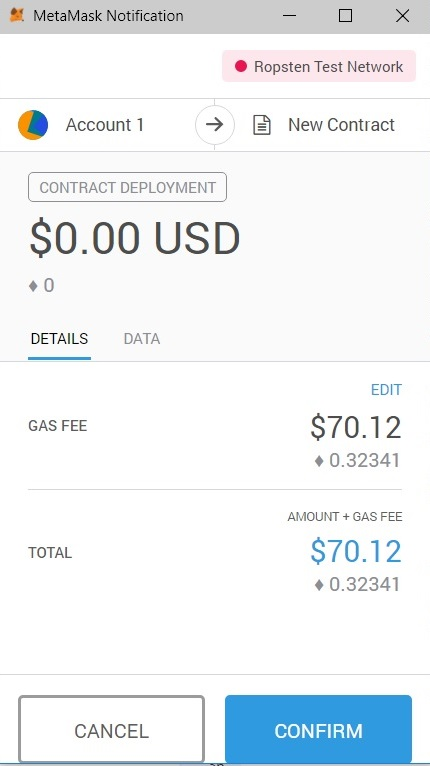
\includegraphics[width=60mm,scale=0.5]{figs/STC}
	\caption{Deploploying Shipment Tracker contract using MetaMask}
	\label{fig:STC} 
\end{figure}
\subsubsection{Cost of Storage on the Blockchain}
In \ref{IPFS} it was mentioned that it becomes prohibitively expensive to store large chunks of data on the blockchain. Table \ref{table:t4} shows the cost of storage on the Ethereum blockchain. This table takes the best case scenario into consideration. In this scenario the minimum observed Eth price was used for calculation. We are only interested in logging values from one sensor, and additionally the log interval is quite large I.e. once every 1 hour. In reality we want our system to have in depth logs of each and every activity and the logging interval should be as small as possible. During IPFS testing we kept the logging interval at 5 minutes. This table makes it obvious it is not feasible to store logging information in the blockchain. 
\begin{table}[h]
\centering
\resizebox{\columnwidth}{!}{%
\begin{tabular}{|c|c|c|c|c|c|c|}
\cline{1-5} \cline{7-7}
\rowcolor[HTML]{5B82BA} 
{\color[HTML]{FFFFFF} \textbf{Data size}}                                     & {\color[HTML]{FFFFFF} \textbf{Gas Required}} & {\color[HTML]{FFFFFF} \textbf{\begin{tabular}[c]{@{}c@{}}Transaction Cost\\ (Eth)\end{tabular}}} & {\color[HTML]{FFFFFF} \textbf{ETH  Price}} & \multicolumn{1}{l|}{\cellcolor[HTML]{5B82BA}{\color[HTML]{FFFFFF} \textbf{Interval}}} & \multicolumn{1}{l|}{\cellcolor[HTML]{5B82BA}{\color[HTML]{FFFFFF} \textbf{Sensors}}} & \multicolumn{1}{l|}{\cellcolor[HTML]{5B82BA}{\color[HTML]{FFFFFF} \textbf{\begin{tabular}[c]{@{}l@{}}Daily Cost\\ (Eth*Eth Price*24)\end{tabular}}}} \\ \hline
\textbf{256 bit word}                                                         & 20000                                        & 0.0006                                                                                           &                                            &                                                                                       &                                                                                      & 3.1968\$                                                                                                                                             \\ \cline{1-3} \cline{7-7} 
\textbf{\begin{tabular}[c]{@{}c@{}}1MB \\ (31250 256-bit words)\end{tabular}} & 625000000                                    & 18.75                                                                                            &                                            &                                                                                       &                                                                                      & 99,900\$                                                                                                                                             \\ \cline{1-3} \cline{7-7} 
\textbf{10MB}                                                                 & 6250000000                                   & 187.5                                                                                            &                                            &                                                                                       &                                                                                      & 999,0000\$                                                                                                                                           \\ \cline{1-3} \cline{7-7} 
\textbf{100MB}                                                                & 62500000000                                  & 1875                                                                                             & \multirow{-4}{*}{222\$}                    & \multirow{-4}{*}{1 hr}                                                                & \multirow{-4}{*}{1}                                                                  & 9,990,000\$                                                                                                                                          \\ \hline
\end{tabular}%
}
\caption {Cost of Storage on Ethereum Blockchain}
\label{table:t4}
\end{table}

\subsubsection{Cost of storing Violations and Requirements}
Sending violations or Requirements to the Shipment Tracker contract takes almost equivalent amount of gas. For the calculations shown in table \ref{table:t4} we used a transaction generated from the Master Node. The transaction was used to set temperature requirements for the IoT node. The gas price for this transaction was kept at 20 gwei. This transaction spent 0.00484134 Eth worth of gas. Which is equivalent to 1 dollar according to the Eth pricing as of 17 August 2018. Alternatively, if we take into account Eth pricing from January, the cost of this transaction becomes 5 dollars.  Our tests have shown that sending violations to the blockchain takes almost the same amounts of gas. The table \ref{table:t4} given below shows daily operational cost based on best case and worst case scenarios. The worst case simulates violations issued for all four sensors attached to the IoT Node. In this case we are only storing each type of violation once, repeated violations will be stored in IPFS. The worst case also simulates a large organization with multiple suppliers and multiple shipments on route at the same time. The table calculations are based on 5 parallel supply lines.

\begin{table}[h]
\centering
\resizebox{\columnwidth}{!}{%
\begin{tabular}{|c|c|c|c|c|c|c|}
\hline
\rowcolor[HTML]{5B82BA} 
{\color[HTML]{FFFFFF} \textbf{}} & {\color[HTML]{FFFFFF} \textbf{Number of Violations}} & {\color[HTML]{FFFFFF} \textbf{Transaction Cost}} & {\color[HTML]{FFFFFF} \textbf{Gas Price}} & {\color[HTML]{FFFFFF} \textbf{Price of 1 ETH}} & \multicolumn{1}{l|}{\cellcolor[HTML]{5B82BA}{\color[HTML]{FFFFFF} \textbf{Number of Supply lines}}} & \multicolumn{1}{l|}{\cellcolor[HTML]{5B82BA}{\color[HTML]{FFFFFF} \textbf{Daily Cost}}} \\ \hline
\textbf{Best Case}               & 0                                                    & 0\$                                              &                                           &                                                & 1                                                                                                   & 0\$                                                                                     \\ \cline{1-3} \cline{6-7} 
\textbf{Worst Case}              & 4                                                    & 1\$                                              & \multirow{-2}{*}{20 gwei}                 & \multirow{-2}{*}{222\$}                        & \textgreater{}5                                                                                     & 20\$                                                                                    \\ \hline
\textbf{Best Case}               & 0                                                    & 0\$                                              &                                           &                                                & 1                                                                                                   & 0                                                                                       \\ \cline{1-3} \cline{6-7} 
\textbf{Worst Case}              & 4                                                    & 4\$                                              & \multirow{-2}{*}{20 gwei}                 & \multirow{-2}{*}{1200\$}                       & \textgreater{}5                                                                                     & 80\$                                                                                    \\ \hline
\end{tabular}%
}
\label{table:t5}
\caption{Daily Operational Cost}
\end{table}
